%
%% SPDX-License-Identifier: CC-BY-NC-SA-4.0
%%

\documentclass[10pt,a4paper,twoside,american]{article}
\usepackage{geometry}
\geometry{verbose,a4paper,tmargin=2cm,bmargin=2cm,lmargin=2cm,rmargin=2cm}
\usepackage[]{float}
\usepackage[table]{xcolor}
\definecolor{shadecolor}{gray}{0.9}
\usepackage{amsmath}
\usepackage{amssymb}
\usepackage{mathtools}
\usepackage{bm}
\usepackage{natbib}
\usepackage{diagbox}
\usepackage[%%
breaklinks=true,
colorlinks=true,
linkcolor=blue,citecolor=blue,urlcolor=blue,filecolor=blue,
pdffitwindow,
bookmarks=true,
bookmarksopen=true,
bookmarksnumbered=true,
pdftitle={},
pdfauthor={},
pdfsubject={},
pdfkeywords={}
]
{hyperref}
\usepackage{enumitem}
%\usepackage{units}
\usepackage{multirow}

\renewcommand\familydefault{cmss}

\usepackage{cleveref}

%%%%%%%%%%%%%%%%%%%%%%%%%%%%%%%%%%%%%%%%%%%%%%%%%%%%%%%%
%% configuration of model-component definitions
\usepackage{amsthm}
\crefformat{definition}{$^\text{#2#1#3}$}
\Crefformat{definition}{$^\text{#2#1#3}$}
%%
\newtheoremstyle{definitionstyle}{2ex}{2ex}{}{0ex}{}{\!}{ }{$^\text{\thmnumber{#2}}$}
\theoremstyle{definitionstyle}
\newtheorem{definition}{}

%%%%%%%%%%%%%%%%%%%%%%%%%%%%%%%%%%%%%%%%%%%%%%%%%%%%%%%%%%%%%%%%%%%%%%%%%%%%%%%%%%%%
%% macros
\newcommand{\diff}{\ensuremath{\text{d}}}
\newcommand{\dtsim}{\Delta t}
\newcommand{\Epop}{\mathcal{E}} %% set (hence caligraphic) of excitatory neurons
\newcommand{\exc}{\text{E}}     %% label for ``excitatory'
\newcommand{\ext}{\text{X}}   %% label for ``external''
\newcommand{\inh}{\text{I}}     %% label for ``inhibitory''
\newcommand{\Ipop}{\mathcal{I}} %% set (hence caligraphic) of inhibitory neurons
\newcommand{\leak}{\text{L}}              %% label for ``external''
\newcommand{\ms}{\,\text{ms}}
\newcommand{\MOhm}{\,\text{M}\Omega}
\newcommand{\mV}{\,\text{mV}}
\newcommand{\nS}{\,\text{nS}}
\newcommand{\pF}{\,\text{pF}}
\newcommand{\pA}{\,\text{pA}}
\newcommand{\RM}{R_\text{m}}
\newcommand{\CM}{C_\text{m}}
\newcommand{\sps}{\,\text{s}^{-1}}
\newcommand{\Stimulus}{\mathcal{S}} %% set (hence caligraphic) of external spike-train generators
\newcommand{\tauM}{\tau_\text{m}}
\newcommand{\tauR}{\tau_\text{ref}}
\newcommand{\tauS}{\tau_\text{s}}
\newcommand{\note}[1]{\textcolor{red}{[\it #1]}}
\newcommand{\drvd}[1]{\textcolor{gray}{#1}} %% font style for derived parameters

%%%%%%%%%%%%%%%%%%%%%%%%%%%%%%%%%%%%%%%%%%%%%%%%%%%%%%%%%%%%%%%%%%%%%%%%%%%%%%%%%%%% 
\begin{document}

\title{Detailed description of the \\ cortical microcircuit model \citep{Potjans14}}
\author{}
\date{last update: \today}
\maketitle
\thispagestyle{empty}
%%%%%%%%%%%%%%%%%%%%%%%%%%%%%%%%%%%%%%%%%%%%%%%%%%%%%%%%%%%%%%%%%%%%%%%%%%%%%%%%%%%%

\def\marg{1ex}
\setlength{\parindent}{0pt}

\tableofcontents
\clearpage
%%%%%%%%%%%%%%%%%%%%%%%%%%%%%%%%%%%%%%%%%%%%%%%%%%%%%%%%%%%%%%%%%%%%%%%%%%%%%%%%%%%%
%%%%%%%%%%%%%%%%%%%%%%%%%%%%%%%%%%%%%%%%%%%%%%%%%%%%%%%%%%%%%%%%%%%%%%%%%%%%%%%%%%%%
\section{Model description}
\label{sec:model_description}
%%%%%%%%%%%%%%%%%%%%%%%%%%%%%%%%%%%%%%%%%%%%%%%%%%%%%%%%%%%%%%%%%%%%%%%%%%%%%%%%%%%%
%% model description table: Summary and Populations
%%
\begin{table}[H]
\renewcommand{\arraystretch}{1.2}
%%%%%%%%%%%%%%%%%%%
\begin{tabular}{
  |@{\hspace*{\marg}}p{0.2\textwidth-2.\marg}@{\hspace*{\marg}}
  |@{\hspace*{\marg}}p{0.8\textwidth-2.\marg}@{\hspace*{\marg}}
  |}
  \hline 
  \multicolumn{2}{|>{\color{white}\columncolor{black}}c|}{\textbf{Summary}}\\
  \hline 
  \textbf{Populations} & $8$ cortical populations in $4$ layers ($\text{L2/3}$, $\text{L4}$, $\text{L5}$,
  $\text{L6}$), driven by a thalamic population ($\mathcal{T}$) and cortico-cortical inputs ($\mathcal{C}$)\\
  \hline 
  \textbf{Connectivity} & random, independent, population specific\\
  \hline 
  \textbf{Neuron model} & cortex: leaky integrate-and-fire (LIF); thalamus, cortico-cortical inputs: Poisson point process\\
  \hline 
  \textbf{Synapse model} & exponential postsynaptic currents with static, normally distributed weights and delays\\
  \hline 
  \textbf{Predictions} & population specific spiking activity\\

  \hline
  \multicolumn{2}{|c|}{\centering\parbox{0.95\linewidth}{\centering
  %%
  %% \includegraphics{figures/NetworkSketch_microcircuit-PD14-model.pdf}\\[-5ex]
  %%
  %% with this, the tex file cannot be compiled locally:
  \includegraphics{docs/model_description/figures/NetworkSketch_microcircuit-PD14-model.pdf}\\[-5ex]
  %%
  \hfill (see \href{https://doi.org/10.1371/journal.pcbi.1010086.g008}{legend})}}\\
  \hline
\end{tabular}
%%%%%%%%%%%%%%%%%%% 
\begin{tabular}{
  |@{\hspace*{\marg}}p{0.4\textwidth-2.\marg}@{\hspace*{\marg}}
  |@{\hspace*{\marg}}p{0.4\textwidth-2.\marg}@{\hspace*{\marg}}
  |@{\hspace*{\marg}}p{0.2\textwidth-2.\marg}@{\hspace*{\marg}}
  |}
  \hline 
  \multicolumn{3}{|>{\color{white}\columncolor{black}}c|}{\textbf{Populations}}\\
  \hline 
  \textbf{Name} & \textbf{Elements} & \textbf{Size}\\
  \hline 
   $x \in \{\mathcal{E}_{23},\mathcal{E}_{4},\mathcal{E}_{5},\mathcal{E}_{6},\mathcal{I}_{23},\mathcal{I}_{4},\mathcal{I}_{5},\mathcal{I}_{6}\}$ & LIF & $N_{x}$\\
  \hline 
  $\mathcal{P} = \bigcup_{x} x$ & LIF & $N= \sum_{x} N_{x}$ (see remark \ref{remark:downscaling})\\
  \hline 
   $\mathcal{T}$ & realizations of Poisson point process & $N_{\mathcal{T}}$ \\
   \hline
   $\mathcal{C}=\bigcup_{x}\mathcal{C}_{x}$ & population specific currents & $N= \sum_{x} N_{x}$
   \\
  \hline 
\end{tabular}
%%%%%%%%%%%%%%%%%%%
\caption{Description of the network model (continued on next page).}
\label{tab:model_description}
\end{table}
\clearpage
%%%%%%%%%%%%%%%%%%%%%%%%%%%%%%%%%%%%%%%%%%%%%%%%%%%%%%%%%%%%%%%%%%%%%%%%%%%%%%%%%%%%
%% model description table (continued): Connectivity
%%
\addtocounter{table}{-1}
\begin{table}[H]
%%%%%%%%%%%%%%%%%%%
%%%%%%%%%%%%%%%%%%% 
\begin{tabular}{
  |@{\hspace*{\marg}}p{0.2\textwidth-2.\marg}@{\hspace*{\marg}}
  |@{\hspace*{\marg}}p{0.2\textwidth-2.\marg}@{\hspace*{\marg}}
  |@{\hspace*{\marg}}p{0.6\textwidth-2.\marg}@{\hspace*{\marg}}
  |}
  \hline 
  \multicolumn{3}{|>{\color{white}\columncolor{black}}c|}{
  \textbf{Connectivity}
  }\\
  \hline 
	\textbf{Source} & \textbf{Target} & \textbf{Pattern}\\
  \hline
   $x \in \{\mathcal{E}_{23},\ldots,\mathcal{I}_{6}\}$ & $y \in \{\mathcal{E}_{23},\ldots,\mathcal{I}_{6}\}$ &
                            \begin{itemize}[align=left,leftmargin=*]
				    \item random, fixed total number $K_{yx}$ of connections\cref{def:random_fixed_total_number} (see remark \ref{remark:downscaling})
                            \item synaptic weights $J_{ij}$ ($\forall{}i\in y, j\in x$)
                            \item spike-transmission delays $d_{ij}$ ($\forall{}i\in y, j\in x$)
                            \end{itemize}\\
  \hline
  $\mathcal{T}$ & $y \in \{\mathcal{E}_{23},\ldots,\mathcal{I}_{6}\}$ &
                            \begin{itemize}[align=left,leftmargin=*]
				    \item random, fixed total number $K_{y\mathcal{T}}$ of connections\cref{def:random_fixed_total_number} 
                            \item synaptic weights $J_{ij}$ ($\forall{}i\in y, j\in \mathcal{T}$)                            \item spike-transmission delays $d_{ij}$ ($\forall{}i\in y, j\in \mathcal{T}$)
                            \end{itemize}\\
  \hline
  $\mathcal{C}_{y}$ & $y \in \{\mathcal{E}_{23},\ldots,\mathcal{I}_{6}\}$ & 
                            \begin{itemize}[align=left,leftmargin=*]
				                    \item one-to-one\cref{def:one_to_one}
                            %\item synaptic weights $J_{ij}$ ($\forall{}i\in y, j\in \mathcal{C}_{y}$)
                            %\item spike-transmission delays $d_{ij}$ ($\forall{}i\in y, j\in \mathcal{C}_{y}$)
                            \end{itemize}\\
  \hline
  %\multicolumn{3}{|p{\linewidth}|}{total number of connections between populations $x$ and $y$: 
  %\begin{equation*} 
    %K_{yx} = \frac{\text{ln}\left(1-C_{yx}\right)}{\text{ln}\left(1-\left(N_{x}N_{y}\right)^{-1}\right)},
  %\end{equation*}
	%with population sizes $N_{x}$, $N_{y}$ and connection probabilities $C_{yx}$.}\\
  %\hline
  \multicolumn{3}{|p{0.95\linewidth}|}{%
  % \remark{footnote:indegree}\textit{random fixed in-degree:} each neuron in $\mathcal{T}$ is connected to $K_\text{in}$ neurons in $\mathcal{S}$ randomly and independently chosen with replacement.
  %%
  \vspace{-1ex}
  Connectivity patterns:
  \begin{definition}
    \label{def:random_fixed_total_number}
    \emph{random, fixed total number} ($N_\text{Syn}$):
	  This rule establishes a total number of
	  \begin{equation*}
		  K_{yx} = \frac{\text{ln}\left(1-C_{yx}\right)}{\text{ln}\left(1-\left(N_{x}N_{y}\right)^{-1}\right)},
	  \end{equation*}
	  connections between a source population $x$ of size $N_x$ and a target population $y$ of size $N_y$.
          $C_{yx}$ denotes the connection probability.
          Sources and targets are randomly and independently drawn from $x$ and $y$ with replacement.
	  Multiple connections between two neurons and self-connections are permitted ($\mathbb{M}$, $\mathbb{A}$).
          %%
          % This rule establishes exactly
	  % \begin{equation*}
	  %         K_{yx} = \frac{\text{ln}\left(1-C_{yx}\right)}{\text{ln}\left(1-\left(N_{x}N_{y}\right)^{-1}\right)},
	  % \end{equation*}
	  % connections between randomly and independently chosen sources in population $x$ with size $N_{x}$ and targets in population $y$ with size $N_{y}$ (with replacement).
	  % The connection probabilities are denoted by $C_{yx}$.
	  % Multiple connections between two neurons and self-connections are permitted ($\mathbb{M}$, $\mathbb{A}$).
  \end{definition}
  \begin{definition}
    \label{def:one_to_one}
    \emph{one-to-one} ($\delta$):
    Each neuron in the source population is connected to one corresponding neuron in the target population (bijection).
  \end{definition}
  \hfill(see ``Network sketch'' above and \citealp{Senk22_e1010086})
}\\

  %\hline

  %\multicolumn{3}{|l|}{self-connections (``autapses'') and multiple connections (``multapses'') are permitted}\\
  \hline

\end{tabular}
%%%%%%%%%%%%%%%%%%%
\caption{Description of the network model (continued).}
\label{tab:model_description_1}
\end{table}
\clearpage
%%%%%%%%%%%%%%%%%%%%%%%%%%%%%%%%%%%%%%%%%%%%%%%%%%%%%%%%%%%%%%%%%%%%%%%%%%%%%%%%%%%%
%% model description table: Neurons
%%
\begin{table}[H]
\renewcommand{\arraystretch}{1.2}
%%%%%%%%%%%%%%%%%%% 
\begin{tabular}{
  |@{\hspace*{\marg}}p{0.2\textwidth-2.\marg}@{\hspace*{\marg}}
  |@{\hspace*{\marg}}p{0.8\textwidth-2.\marg}@{\hspace*{\marg}}
  |}
  \hline 
  \multicolumn{2}{|>{\color{white}\columncolor{black}}c|}{\textbf{Neurons}}\\
  \hline
  \multicolumn{2}{|>{\color{black}\columncolor{lightgray}}c|}{\textbf{Cortical neurons}}\\
  \hline
  \textbf{Type} & leaky integrate-and-fire (LIF)\\
  \hline 
  \textbf{Description} & dynamics of membrane potential $V_{i}(t)$ and spiking activity $s_i(t)$ of neuron $i\in x$ for $x\in\{\mathcal{E}_{23},\ldots,\mathcal{I}_{6}\}$:
                         \begin{itemize}
                         \item emission of $k$th ($k=1,2,\ldots$) spike of neuron $i$ at time $t_{i}^{k}$ if
                           \begin{equation*}
                             V_{i}\left(t_{i}^{k}\right)\geq\theta  
                           \end{equation*}
                           with spike threshold $\theta$
                         \item reset and refractoriness:
                           \begin{equation*}
				   \forall{}k,\ \forall t \in \left[t_{k}^{i},\,t_{k}^{i}+\tauR\right]:\quad V_{i}(t)=V_\text{reset}  
                           \end{equation*}
                            with refractory period $\tauR$ and reset potential $V_\text{reset}$
                         \item spike train $\displaystyle s_i(t)=\sum_k \delta(t-t_i^k)$
                         \item subthreshold dynamics of membrane potential $V_{i}(t)$:
                           \begin{equation}
			     \label{eq:membrane_potential}
                             \begin{aligned}
                               &\forall{}k,\ \forall t \notin \left[t_{i}^{k},\,t_{i}^{k}+\tauR\right):\\
                               &\qquad\tauM\frac{\diff{}V_i(t)}{\diff{}t} =
                               \Bigl[E_\text{L}-V_i(t)\Bigr]+\RM I_i(t)
                             \end{aligned}
                           \end{equation}
                           with membrane time constant $\tauM$, membrane resistance $\RM$, resting potential $E_\text{L}$, and total synaptic input current $I_i(t)$
                         \end{itemize}\\
  \hline 
  \multicolumn{2}{|>{\color{black}\columncolor{lightgray}}c|}{\textbf{Thalamic neurons}}\\
  \hline
  \textbf{Type} & Poisson point process \\
  \hline 
  \textbf{Description} &  spike trains $s_{i}(t)$ ($i\in\mathcal{T}$) modeled as independent realizations of Poisson point process with piece-wise constant rate
  \begin{equation*}
      \nu_{\mathcal{T}}(t) = \nu_{\mathcal{T}}\cdot\left(\Theta(t-t_{\text{start}})-\Theta(t-t_{\text{stop}})\right)
  \end{equation*}\\
  \hline
  \multicolumn{2}{|>{\color{black}\columncolor{lightgray}}c|}{\textbf{Cortico-cortical inputs}}\\
  \hline
  \textbf{Type} & constant (direct) currents (DC) \\
  \hline 
	\textbf{Description} & population specific constant input current of magnitude
\begin{equation*}
	I_{\mathcal{C}_x} = K_{\mathcal{C}_x} \cdot I_{\mathcal{C}}
  \quad (\forall x\in\{\mathcal{E}_{23},\ldots,\mathcal{I}_{6}\})\, ,
\end{equation*}
	with cortico-cortical in-degree $K_{\mathcal{C}_x}$, and mean current
  \begin{equation*}
    I_{\mathcal{C}} = \nu_{\mathcal{C}} \cdot \bar{I}_{y,\mathcal{C}}\cdot\tauS \quad (\forall y\in\{\mathcal{E}_{23}, \dots, \mathcal{I}_{6}\})
  \end{equation*}
    generated by a Poissonian spike train with rate $\nu_{\mathcal{C}}$, convolved with an exponential kernel with amplitude $\bar{I}_{y, \mathcal{C}}$ and time constant $\tauS$ (see remark \ref{remark:DC_stim})
  \\
  \hline
  
\end{tabular}
%%%%%%%%%%%%%%%%%%%
\caption{Description of the network model (continued).}
\label{tab:model_description_2}
\end{table}
\clearpage
%%%%%%%%%%%%%%%%%%%%%%%%%%%%%%%%%%%%%%%%%%%%%%%%%%%%%%%%%%%%%%%%%%%%%%%%%%%%%%%%%%%%
%% model description table: Synapses
%%
\begin{table}
\begin{tabular}{
  |@{\hspace*{\marg}}p{0.2\textwidth-2.\marg}@{\hspace*{\marg}}
  |@{\hspace*{\marg}}p{0.8\textwidth-2.\marg}@{\hspace*{\marg}}
  |}
  \hline 
  \multicolumn{2}{|>{\color{white}\columncolor{black}}c|}{
  \textbf{Synapses}
  }\\
  \hline 
  \textbf{Type} & exponential postsynaptic currents with static weights and delays \\
  \hline 
  \textbf{Description} &
  \begin{itemize}
	  %\item total synaptic input current $I_{ij}(t)$ from neuron $j$ to neuron $i$ ($\forall i \in y\in\{\mathcal{E}_{23},\ldots,\mathcal{I}_{6}\}$ and $\forall j \in x\in\{\mathcal{E}_{23},\ldots,\mathcal{I}_{6}, \mathcal{T}, \mathcal{C}\}$):
	\item total synaptic input current $I_i(t)$ to neuron $i$ ($\forall i \in y\in\{\mathcal{E}_{23},\ldots,\mathcal{I}_{6}\}$) is governed by:
		\begin{equation}
			\label{eq:synaptic_current}
			\left(\frac{\diff}{\diff t} + \frac{1}{\tauS}\right) I_{i} (t) = f_{i}(t)
		\end{equation}
		with superposition from all neurons $j \in x,\;\forall x\in\{\mathcal{E}_{23},\ldots,\mathcal{I}_{6}, \mathcal{T}, \mathcal{C}\}$
		\begin{equation*}
			f_{i} (t) = \sum_{x} \sum_{j} f_{ij} (t) = \sum_{x} \sum_{j} \hat{I}_{ij} s_{j}(t-d_{ij})
		\end{equation*}
		  of weighted spike trains with static synaptic weigths $\hat{I}_{ij}$, synaptic time constant $\tauS$, and spike transmission delays $d_{ij}$
		
  %\begin{equation*}
      %I_{i}(t) = \sum_{j} J_{ij} \left(h * s_{j}\right)(t-d_{ij}),
  %\end{equation*}
  %with 
  %\begin{itemize}
	\item solution of \eqref{eq:synaptic_current} for $\displaystyle f_{ij}(t)=\hat{I}_{ij}s_{j}(t)$ and $I_{ij}(t=0)=0$:
		\begin{equation*}
			\text{PSC}_{ij}(t)=\hat{I}_{ij} \exp(-t/\tauS)\Theta(t)
		\end{equation*}
		with Heaviside function $\Theta(\cdot)$
	\item[$\curvearrowright$] (exponential decaying) posynaptic current triggered by a single presynaptic spike 
	\item solution of \eqref{eq:membrane_potential} for $I_i(t)=\text{PSC}_{ij}(t)$, $V_i(t=0)=0$, and $E_\text{L}=0$:
                           \begin{equation*}
                             \text{PSP}_{ij}(t)=
				     \hat{I}_{ij}\RM \frac{\tauS}{\tauS - \tauM}
				     \left(e^{-t/\tauS}-e^{-t/\tauM}\right) \Theta(t) 
                           \end{equation*}
                         \item PSC amplitude (synaptic weight):
                           \begin{equation*}                          
                             \hat{I}_{ij}
                             =\frac{J_{ij}}{J_\text{unit}(\tauM,\tauS,\RM)}
                           \end{equation*}
                           parameterized by PSP amplitude                    
                           $J_{ij}=\text{max}_t\bigl(\text{PSP}_{ij}(t)\bigr)$ 
                         \item[] with unit PSP amplitude (PSP amplitude for $\hat{I}_{ij}=1$):
                           \begin{equation*}
                             J_\text{unit}(\tauM,\tauS,\RM)=
				   \RM\frac{\tauS}{\tauS-\tauM} \left( \left[ \frac{\tauM}{\tauS} \right]^{-\tauM/(\tauM - \tauS)} - \left[ \frac{\tauM}{\tauS} \right]^{-\tauS/(\tauM-\tauS)} \right)
                           \end{equation*}
                         \item[] and time to PSP maximum:
                           \begin{equation*}
                             t_\text{max} =
				   \frac{\tauS\tauM}{\tauM - \tauS} \ln\left(\frac{\tauM}{\tauS}\right)
                           \end{equation*}
  \end{itemize}\\
  \hline
\end{tabular}
%%%%%%%%%%%%%%%%%%%
\caption{Description of the network model (continued).}
\label{tab:model_description_2}
\end{table}
\clearpage
%%%%%%%%%%%%%%%%%%%%%%%%%%%%%%%%%%%%%%%%%%%%%%%%%%%%%%%%%%%%%%%%%%%%%%%%%%%%%%%%%%%% 
%% model description table: Synapses (cnt) and Initial conditions
%%
\begin{table}
\begin{tabular}{
  |@{\hspace*{\marg}}p{0.2\textwidth-2.\marg}@{\hspace*{\marg}}
  |@{\hspace*{\marg}}p{0.8\textwidth-2.\marg}@{\hspace*{\marg}}
  |}
  \hline 
  \multicolumn{2}{|>{\color{white}\columncolor{black}}c|}{
	  \textbf{Synapses (continued)}
  }\\
  \hline 
  \textbf{Description} &
  \begin{itemize}
  \item synaptic weights
  \begin{equation*}
	  \hat{I}_{ij} = \begin{cases} 
      \text{max}(0,z_{yx}), & j \in x\in\{\mathcal{E}_{23},\mathcal{E}_{4},\mathcal{E}_{5},\mathcal{E}_{6},\mathcal{T}\} \\
      \text{min}(0,z_{yx}), & j \in x\in\{\mathcal{I}_{23},\mathcal{I}_{4},\mathcal{I}_{5},\mathcal{I}_{6}\} \\
      \bar{I}_{yx}, & j \in x=\mathcal{C} \\
      \end{cases}
  \end{equation*}
  with
  \begin{equation*}
      z_{yx} \sim\mathcal{N}\left\{\bar{I}_{yx},\,\sigma_{\text{s},yx}^2\right\}
  \end{equation*}
  drawn from a normal distribution with mean $\bar{I}_{yx}$, variance $\sigma_{\text{s},yx}^2$
  \item[] note: clipping of synaptic weights leads to a deviation of the total number of synapses with non-zero weights from $K_{yx}$ (see ``Connectivity'')
  \item distributed synaptic delays
  \begin{equation*}
      d_{ij} = \begin{cases} 
	      \text{max}(d_\text{min},z_{x}), & j \in x\in\{\mathcal{E}_{23},\ldots,\mathcal{I}_{6},\mathcal{T}\} \\
      	\bar{d}_{x}, & j \in x=\mathcal{C} \\
      \end{cases}
  \end{equation*}
  with
  \begin{equation*}
      z_{x} \sim\mathcal{N}\left\{\bar{d}_{x},\,\sigma_{\text{d},x}^2\right\}
  \end{equation*}
  drawn from a normal distribution with mean $\bar{d}_{x}$, variance $\sigma_{\text{d},x}^2$, and minimal delay $d_\text{min} > 0$
  \end{itemize}\\
  \hline
\end{tabular}
%%%%%%%%%%%%%%%%%%%
\begin{tabular}{
  |@{\hspace*{\marg}}p{0.2\textwidth-2.\marg}@{\hspace*{\marg}}
  |@{\hspace*{\marg}}p{0.8\textwidth-2.\marg}@{\hspace*{\marg}}
  |}
  \hline
  \multicolumn{2}{|>{\color{white}\columncolor{black}}c|}{
  \textbf{Initial conditions}
  }\\
\hline
\textbf{Type} & random initial membrane potentials and homogeneous initial synaptic currents\\
\hline
  \textbf{Description} &
  \begin{itemize}
  \item membrane potentials
    \begin{equation*}
      V_i(t=0)\sim\mathcal{N}(\bar{V}_{0,x},\sigma_{\text{v},x}^2)
    \end{equation*}
  randomly and independently drawn from a normal distribution with mean $\bar{V}_{0,x}$ and variance $\sigma^2_{\text{v},x}$ ($\forall i \in x\in\{\mathcal{E}_{23},\ldots,\mathcal{I}_{6}\}$; see remark \ref{remark:initial_conditions})
  \item synaptic currents: $I_{i}(t=0)=0\,\text{pA}$ ($\forall i \in y\in\{\mathcal{E}_{23},\ldots,\mathcal{I}_{6}\}$)
  \end{itemize}\\
  \hline
\end{tabular}
%%%%%%%%%%%%%%%%%%%
\caption{Description of the network model (continued).}
\end{table}
\clearpage
%%%%%%%%%%%%%%%%%%%%%%%%%%%%%%%%%%%%%%%%%%%%%%%%%%%%%%%%%%%%%%%%%%%%%%%%%%%%%%%%%%%%
%%%%%%%%%%%%%%%%%%%%%%%%%%%%%%%%%%%%%%%%%%%%%%%%%%%%%%%%%%%%%%%%%%%%%%%%%%%%%%%%%%%%
\section{Model parameters}
\label{sec:model_parameters}
%%
\renewcommand{\arraystretch}{1.2}
%%
%% parameters table
\def\widthA{0.1}
\def\widthB{0.2}
\def\widthC{0.7}
\begin{table}[H]
%%%%%%%%%%%%%%%%%%%
%%%%%%%%%%%%%%%%%%% 
%% the following parameters are implementation details; this doesn't belong to the model description
  % \begin{tabular}{|@{\hspace*{1mm}}p{0.1\linewidth}@{}|@{\hspace*{1mm}}p{0.2\linewidth}|@{\hspace*{1mm}}p{0.665\linewidth}|}
% \hline 
% \multicolumn{3}{|>{\color{white}\columncolor{black}}l|}{\textbf{A: Global simulation parameters}}\\
% \hline 
% \textbf{Symbol} & \textbf{Value} & \textbf{Description}\\
% \hline 
% $T_{\text{sim}}$ & $\unit[10,000]{ms}$ & Simulation duration\\
% $dt$ & $\unit[0.1]{ms}$ & Temporal resolution\\
% $T_{\text{trans}}$ & $\unit[1,000]{ms}$ & Startup transient\\
% \hline 
% \end{tabular}

% \begin{tabular}{|@{\hspace*{1mm}}p{0.1\linewidth}@{}|@{\hspace*{1mm}}p{0.2\linewidth}|@{\hspace*{1mm}}p{0.665\linewidth}|}
% \hline 
% \multicolumn{3}{|>{\color{white}\columncolor{black}}l|}{\textbf{B: Preprocessing}}\\
% \hline 
% \textbf{Symbol} & \textbf{Value} & \textbf{Description}\\
% \hline 
% $\Delta t$ & $\unit[0.5]{ms}$ & Temporal bin size\\
% \hline 
% \end{tabular}

  %\begin{tabular}{|@{\hspace*{1mm}}p{0.99\linewidth}|}
  \begin{tabular}{|@{\hspace*{\marg}}p{1.0\textwidth-2.\marg}@{\hspace*{\marg}}|}
  %% \begin{tabular}{
  %%   |@{\hspace*{\marg}}p{\widthA\textwidth-2.\marg}@{\hspace*{\marg}}
  %%   |@{\hspace*{\marg}}p{\widthB\textwidth-2.\marg}@{\hspace*{\marg}}
  %%   |@{\hspace*{\marg}}p{\widthC\textwidth-2.\marg}@{\hspace*{\marg}}
  %%   |}
    \hline
    \multicolumn{1}{|>{\color{black}\columncolor{lightgray}}c|}{\textbf{Network and connectivity}}\\
    \hline
    \multicolumn{1}{|>{\color{black}\columncolor{white}}c|}{\textbf{Population sizes}}\\
    \hline
    \\
    \multicolumn{1}{|c|}{
      \begin{tabular}{|p{6ex}|p{6ex}|p{6ex}|p{6ex}|p{6ex}|p{6ex}|p{6ex}|p{6ex}|p{6ex}|p{6ex}|}
      \hline
      $x$ & $\mathcal{E}_{23}$ & $\mathcal{I}_{23}$ & $\mathcal{E}_{4}$ & $\mathcal{I}_{4}$ & $\mathcal{E}_{5}$ & $\mathcal{I}_{5}$ & $\mathcal{E}_{6}$ & $\mathcal{I}_{6}$ & $\mathcal{T}$\\
      \hline
      $N_{x}$ & $20,683$ & $5,834$ & $21,915$ & $5,479$ & $4,850$ & $1,065$ & $14,395$ & $2,948$ & $902$\\
      \hline
      \end{tabular}
    }\\
    \\
    \hline
    \multicolumn{1}{|>{\color{black}\columncolor{white}}c|}{\textbf{Connection probabilities} $C_{yx}$}\\
    \hline
    \\
    \multicolumn{1}{|c|}{
    \begin{tabular}{|p{6ex}|p{6ex}|p{6ex}|p{6ex}|p{6ex}|p{6ex}|p{6ex}|p{6ex}|p{6ex}|p{6ex}|}
      \hline
      \diagbox[innerwidth=6ex]{$y$}{$x$} & $\mathcal{E}_{23}$ & $\mathcal{I}_{23}$ & $\mathcal{E}_{4}$ & $\mathcal{I}_{4}$ & $\mathcal{E}_{5}$ & $\mathcal{I}_{5}$ & $\mathcal{E}_{6}$ & $\mathcal{I}_{6}$ & $\mathcal{T}$\\
      \hline
      $\mathcal{E}_{23}$ & $0.1009$ & $0.1689$ & $0.0437$ & $0.0818$ & $0.0323$ & $0.0$ & $0.0076$ & $0.0$ & $0.0$\\
      \hline
      $\mathcal{I}_{23}$ & $0.1346$ & $0.1371$ & $0.0316$ & $0.0515$ & $0.0755$ & $0.0$ & $0.0042$ & $0.0$ & $0.0$\\
      \hline
      $\mathcal{E}_{4}$ & $0.0077$ & $0.0059$ & $0.0497$ & $0.1350$ & $0.0067$ & $0.0003$ & $0.0453$ & $0.0$ & $0.0983$\\
      \hline
      $\mathcal{I}_{4}$ & $0.0691$ & $0.0029$ & $0.0794$ & $0.1597$ & $0.0033$ & $0.0$ & $0.1057$ & $0.0$ & $0.0619$\\
      \hline
      $\mathcal{E}_{5}$ & $0.1004$ & $0.0622$ & $0.0505$ & $0.0057$ & $0.0831$ & $0.3726$ & $0.0204$ & $0.0$ & $0.0$\\
      \hline
      $\mathcal{I}_{5}$ & $0.0548$ & $0.0269$ & $0.0257$ & $0.0022$ & $0.0600$ & $0.3158$ & $0.0086$ & $0.0$ & $0.0$\\
      \hline
      $\mathcal{E}_{6}$ & $0.0156$ & $0.0066$ & $0.0211$ & $0.0166$ & $0.0572$ & $0.0197$ & $0.0396$ & $0.2252$ & $0.0512$\\
      \hline
      $\mathcal{I}_{6}$ & $0.0364$ & $0.0010$ & $0.0034$ & $0.0005$ & $0.0277$ & $0.0080$ & $0.0658$ & $0.1443$ & $0.0196$\\
      \hline
    \end{tabular}
    }\\
    \\
    \hline
  \end{tabular}\\
%\begin{tabular}{|@{\hspace*{1mm}}p{0.083\linewidth}@{}@{\hspace*{1mm}}p{0.07\linewidth}|@{\hspace*{1mm}}p{0.07\linewidth}|@{\hspace*{1mm}}p{0.07\linewidth}|@{\hspace*{1mm}}p{0.07\linewidth}|@{\hspace*{1mm}}p{0.07\linewidth}|@{\hspace*{1mm}}p{0.07\linewidth}|@{\hspace*{1mm}}p{0.07\linewidth}|@{\hspace*{1mm}}p{0.07\linewidth}|@{\hspace*{1mm}}p{0.07\linewidth}|@{\hspace*{1mm}}p{0.1\linewidth}|}
%	\hline 
%	\multicolumn{11}{|>{\color{black}\columncolor{lightgray}}c|}{\textbf{Network and connectivity}}\\
%        \hline
%        \multicolumn{11}{|>{\color{black}\columncolor{white}}c|}{\textbf{Population sizes $N_{x}$}}\\
        %\hline
	%\multicolumn{1}{|l|}{\textbf{Name}} & \multicolumn{1}{l}{\textbf{Value}} & \multicolumn{1}{l}{} & \multicolumn{1}{l}{} & \multicolumn{1}{l}{} & \multicolumn{1}{l}{} & \multicolumn{1}{l}{} & \multicolumn{1}{l}{} & \multicolumn{1}{l}{} &  & \textbf{Description}\\
%	\hline 
%	& \multicolumn{1}{c|}{$x$} & $\mathcal{E}_{23}$ & $\mathcal{I}_{23}$ & $\mathcal{E}_{4}$ & $\mathcal{I}_{4}$ & $\mathcal{E}_{5}$ & $\mathcal{I}_{5}$ & $\mathcal{E}_{6}$ & $\mathcal{I}_{6}$ & $\mathcal{T}$ \\
%	\cline{2-11}
%	& \multicolumn{1}{c|}{$N_{x}$} & $20,683$ & $5,834$ & $21,915$ & $5,479$ & $4,850$ & $1,065$ & $14,395$ & $2,948$ & $902$ \\
%       \multicolumn{11}{|c|}{}\\
	%\hline 
	%\multicolumn{1}{|l|}{$K_{x,\text{ext}}$} & $1,600$ & $1,500$ & $2,100$ & $1,900$ & $2,000$ & $1,900$ & $2,900$ & $2,100$ & - & External\newline in-degree\\
%	\hline
%	\multicolumn{11}{|>{\color{black}\columncolor{white}}c|}{\textbf{Connection probabilities $C_{yx}$}}\\
%	\hline 
%	& \multicolumn{10}{c|}{from~$x$}\\
%	&  & $\mathcal{E}_{23}$ & $\mathcal{I}_{23}$ & $\mathcal{E}_{4}$ & $\mathcal{I}_{4}$ & $\mathcal{E}_{5}$ & $\mathcal{I}_{5}$ & $\mathcal{E}_{6}$ & $\mathcal{I}_{6}$ & $\mathcal{T}$\\
%	\cline{2-11} \cline{3-11} \cline{4-11} \cline{5-11} \cline{6-11} \cline{7-11} \cline{8-11} \cline{9-11} \cline{10-11} \cline{11-11} 
%	& $\mathcal{E}_{23}$ & $0.1009$ & $0.1689$ & $0.0437$ & $0.0818$ & $0.0323$ & $0.0$ & $0.0076$ & $0.0$ & $0.0$\\
%	\cline{2-11} \cline{3-11} \cline{4-11} \cline{5-11} \cline{6-11} \cline{7-11} \cline{8-11} \cline{9-11} \cline{10-11} \cline{11-11} 
%	& $\mathcal{I}_{23}$ & $0.1346$ & $0.1371$ & $0.0316$ & $0.0515$ & $0.0755$ & $0.0$ & $0.0042$ & $0.0$ & $0.0$\\
%	\cline{2-11} \cline{3-11} \cline{4-11} \cline{5-11} \cline{6-11} \cline{7-11} \cline{8-11} \cline{9-11} \cline{10-11} \cline{11-11} 
%	& $\mathcal{E}_{4}$ & $0.0077$ & $0.0059$ & $0.0497$ & $0.1350$ & $0.0067$ & $0.0003$ & $0.0453$ & $0.0$ & $0.0983$\\
%	\cline{2-11} \cline{3-11} \cline{4-11} \cline{5-11} \cline{6-11} \cline{7-11} \cline{8-11} \cline{9-11} \cline{10-11} \cline{11-11} 
%	to~$y$ & $\mathcal{I}_{4}$ & $0.0691$ & $0.0029$ & $0.0794$ & $0.1597$ & $0.0033$ & $0.0$ & $0.1057$ & $0.0$ & $0.0619$\\
%	\cline{2-11} \cline{3-11} \cline{4-11} \cline{5-11} \cline{6-11} \cline{7-11} \cline{8-11} \cline{9-11} \cline{10-11} \cline{11-11} 
%	& $\mathcal{E}_{5}$ & $0.1004$ & $0.0622$ & $0.0505$ & $0.0057$ & $0.0831$ & $0.3726$ & $0.0204$ & $0.0$ & $0.0$\\
%	\cline{2-11} \cline{3-11} \cline{4-11} \cline{5-11} \cline{6-11} \cline{7-11} \cline{8-11} \cline{9-11} \cline{10-11} \cline{11-11} 
%	& $\mathcal{I}_{5}$ & $0.0548$ & $0.0269$ & $0.0257$ & $0.0022$ & $0.0600$ & $0.3158$ & $0.0086$ & $0.0$ & $0.0$\\
%	\cline{2-11} \cline{3-11} \cline{4-11} \cline{5-11} \cline{6-11} \cline{7-11} \cline{8-11} \cline{9-11} \cline{10-11} \cline{11-11} 
%	& $\mathcal{E}_{6}$ & $0.0156$ & $0.0066$ & $0.0211$ & $0.0166$ & $0.0572$ & $0.0197$ & $0.0396$ & $0.2252$ & $0.0512$\\
%	\cline{2-11} \cline{3-11} \cline{4-11} \cline{5-11} \cline{6-11} \cline{7-11} \cline{8-11} \cline{9-11} \cline{10-11} \cline{11-11} 
%	& $\mathcal{I}_{6}$ & $0.0364$ & $0.0010$ & $0.0034$ & $0.0005$ & $0.0277$ & $0.0080$ & $0.0658$ & $0.1443$ & $0.0196$\\
 %   \hline
  %\end{tabular}
\begin{tabular}{
    |@{\hspace*{\marg}}p{\widthA\textwidth-2.\marg}@{\hspace*{\marg}}
    |@{\hspace*{\marg}}p{\widthB\textwidth-2.\marg}@{\hspace*{\marg}}
    |@{\hspace*{\marg}}p{\widthC\textwidth-2.\marg}@{\hspace*{\marg}}
    |}
\hline
\multicolumn{3}{|>{\color{black}\columncolor{lightgray}}c|}{\textbf{Neuron}}\\
\hline 
\textbf{Name} & \textbf{Value} & \textbf{Description}\\
\hline
$\theta$ & $-50\mV$ & spike threshold \\
\hline
$E_{\text{L}}$ & $-65\mV$ & resting potential \\
\hline
$\tau_{\text{m}}$ & $10\ms$ & membrane time constant \\
\hline
$C_{\text{m}}$ & $250\pF$ & membrane capacitance \\
\hline
\drvd{$\RM$} & \drvd{$\tauM/C_{\text{m}} = 40\MOhm$} & membrane resistance \\
\hline
$V_{\text{reset}}$ & $-65\mV$ & reset potential \\
\hline
$\tau_{\text{ref}}$ & $2\ms$ & absolute refractory period \\
\hline
$\tau_{\text{s}}$ & $0.5\ms$ & postsynaptic current time constant \\
\hline
$\nu_{\mathcal{T}}$ & $120\sps$ & rate of thalamic neurons \\
\hline
$t_{\text{start}}$ & $700\ms$ & start time of thalamic input\\
\hline
$\Delta{t_{\mathcal{T}}}$ & $10\ms$ & duration of thalamic input \\
\hline
\drvd{$t_{\text{stop}}$} & \drvd{$t_{\text{start}}+\Delta{t_{\mathcal{T}}} = 710\ms$} & stop time of thalamic input\\
\hline
$\nu_{\mathcal{C}}$ & $8\sps$ & rate of cortico-cortical inputs\\
\hline
\drvd{$I_{\mathcal{C}}$} & \drvd{$\nu_{\mathcal{C}}\bar{I}_{y,\mathcal{C}}\tauS = 0.3 \pA$} & mean amplitude of DC inputs ($\forall y\in\{\mathcal{E}_{23}, \dots, \mathcal{I}_{6}\}$)\\
\hline
%\end{tabular}\\
%%%%%%%%%%%%%%%%
%\begin{tabular}{|@{\hspace*{\marg}}p{1.0\textwidth-2.\marg}@{\hspace*{\marg}}|}
  %\hline
    \multicolumn{3}{|>{\color{black}\columncolor{white}}c|}{\textbf{Population specific cortico-cortical in-degree }$K_{\mathcal{C}_{x}}$}\\
    \hline
    %\vspace{-1ex}
    \multicolumn{3}{|c|}{}\\
    \multicolumn{3}{|c|}{
      %\begin{center}
      \begin{tabular}{|p{7ex}|p{7ex}|p{7ex}|p{7ex}|p{7ex}|p{7ex}|p{7ex}|p{7ex}|p{7ex}|p{7ex}|}
      \hline
       $\mathcal{C}_{x}$ & $\mathcal{C}_{\mathcal{E}_{23}}$ & $\mathcal{C}_{\mathcal{I}_{23}}$ & $\mathcal{C}_{\mathcal{E}_{4}}$ & $\mathcal{C}_{\mathcal{I}_{4}}$ & $\mathcal{C}_{\mathcal{E}_{5}}$ & $\mathcal{C}_{\mathcal{I}_{5}}$ & $\mathcal{C}_{\mathcal{E}_{6}}$ & $\mathcal{C}_{\mathcal{I}_{6}}$ & $\mathcal{C}_{\mathcal{T}}$\\
      \hline
      $K_{\mathcal{C}_{x}}$ & $1600$ & $1500$ & $2100$ & $1900$ & $2000$ & $1900$ & $2900$ & $2100$ & $-$\\
      \hline
      \end{tabular}
      %\end{center}
    }\\
    \multicolumn{3}{|c|}{}\\
    \hline
\end{tabular}
\caption{Model parameters (continued on next page).}
\end{table}

\begin{table}[H]
%\begin{tabular}{
		%|@{\hspace*{\marg}}p{1.0\textwidth-2.\marg}@{\hspace*{\marg}}
		%|@{\hspace*{\marg}}p{1.0\textwidth-2.\marg}@{\hspace*{\marg}}
		%|@{\hspace*{\marg}}p{1.0\textwidth-2.\marg}@{\hspace*{\marg}}
		%|}
\begin{tabular}{
    |@{\hspace*{\marg}}p{\widthA\textwidth-2.\marg}@{\hspace*{\marg}}
    |@{\hspace*{\marg}}p{\widthB\textwidth-2.\marg}@{\hspace*{\marg}}
    |@{\hspace*{\marg}}p{\widthC\textwidth-2.\marg}@{\hspace*{\marg}}
    |}
\hline
\multicolumn{3}{|>{\color{black}\columncolor{lightgray}}c|}{\textbf{Synapse}}\\
\hline 
\textbf{Name} & \textbf{Value} & \textbf{Description}\\
\hline 
$J$ & $0.15\mV$ & (mean) weight (PSP amplitude) of excitatory synapses\\
\hline
\drvd{$\bar{I}_{yx}$} &  & synaptic weights:\\
	& \drvd{$J/J_{\text{unit}}\approx 87.81\pA$} & $x\in\left\{ \mathcal{E}_{23}, \mathcal{E}_{4}, \mathcal{E}_{5}, \mathcal{E}_{6},\mathcal{T}, \mathcal{C}\right\} $\\
	& \drvd{$-4J/J_{\text{unit}}$} & $x\in\left\{ \mathcal{I}_{23}, \mathcal{I}_{4}, \mathcal{I}_{5}, \mathcal{I}_{6}\right\}$, except for:\\
	& \drvd{$2J/J_{\text{unit}}$} & $\left(x,y\right)=\left(\mathcal{E}_{23}, \mathcal{E}_{4}\right)$\\
\hline
$\sigma_{\text{s},yx}$ & $0.1\cdot \bar{I}_{yx}$ & standard deviation of weight distribution\\
\hline
$\bar{d}_{x}$ &  & mean spike transmission delays:\\
 & $1.5\ms$ & $x\in\left\{ \mathcal{E}_{23}, \mathcal{E}_{4}, \mathcal{E}_{5}, \mathcal{E}_{6},\mathcal{T},\mathcal{C}\right\} $\\
 & $0.75\ms$ & $x\in\left\{ \mathcal{I}_{23}, \mathcal{I}_{4}, \mathcal{I}_{5}, \mathcal{I}_{6}\right\}$ \\
 \hline
  $\sigma_{\text{d},x}$ & $0.5\cdot\bar{d}_{x}$ & standard deviation of spike transmission delays\\
  \hline
  $d_\text{min}$      & $0.1\ms$      & minimal spike transmission delay\\ 
\hline
%%%%%%%%%%%%%%%%%%%%%%%%%%%%%%%%%%%%%%%%%%%%%%%%%%%
\multicolumn{3}{|>{\color{black}\columncolor{lightgray}}c|}{\textbf{Initial conditions}}\\
\hline
% \multicolumn{3}{|>{\color{black}\columncolor{white}}c|}{\textbf{Original implementation}}\\
% \hline 
% \textbf{Name} & \textbf{Value} & \textbf{Description}\\
% \hline
% \drvd{$V_{0,\text{mean}}$}    & \drvd{$-58.0\,\mV$} & homogeneous mean of the distribution \\
% 	& & of the initial membrane potential \\
% 	& & $V_{0, \text{mean}}^{(y)} = V_{0, \text{mean}} \quad \forall y\in\{\mathcal{E}_{23},\ldots,\mathcal{I}_{6}\}$\\
% \hline
% \drvd{$V_{0,\text{std}}$}    & \drvd{$10.0\,\mV$} & homogeneous standard deviation of the distribution \\ 
% 	& & of the initial membrane potential \\
% 	& & $V_{0, \text{std}}^{(y)} = V_{0, \text{std}} \quad \forall y\in\{\mathcal{E}_{23},\ldots,\mathcal{I}_{6}\}$\\
% \hline
\multicolumn{3}{|>{\color{black}\columncolor{white}}c|}{\textbf{Population specific mean and standard deviation of initial membrane-potential distributions}}\\
\hline
%\vspace{-1ex}
\multicolumn{3}{|c|}{}\\
\multicolumn{3}{|c|}{
%\begin{center}
	\begin{tabular}{|p{14ex}|>{\raggedleft}p{7ex}|>{\raggedleft}p{7ex}|>{\raggedleft}p{7ex}|>{\raggedleft}p{7ex}|>{\raggedleft}p{7ex}|>{\raggedleft}p{7ex}|>{\raggedleft}p{7ex}|>{\raggedleft\arraybackslash}p{7ex}|}
	\hline
	population $x$ & $\mathcal{E}_{23}$ & $\mathcal{I}_{23}$ & $\mathcal{E}_{4}$ & $\mathcal{I}_{4}$ & $\mathcal{E}_{5}$ & $\mathcal{I}_{5}$ & $\mathcal{E}_{6}$ & $\mathcal{I}_{6}$\\
        \hline
	\vspace{-1ex} $\bar{V}_{0, x}$ ($\mV$) & \vspace{-1ex} $-68.28$ & \vspace{-1ex} $-63.16$ & \vspace{-1ex} $-63.33$ & \vspace{-1ex} $-63.45$ & \vspace{-1ex} $-63.11$ & \vspace{-1ex} $-61.66$ & \vspace{-1ex} $-66.72$ & \vspace{-1ex} $-61.45$\\
        \hline
	\vspace{-1ex} $\sigma_{\text{v}, x}$ ($\mV$) & \vspace{-1ex} $5.36$ & \vspace{-1ex} $4.57$ & \vspace{-1ex} $4.74$ & \vspace{-1ex} $4.94$ & \vspace{-1ex} $4.94$ & \vspace{-1ex} $4.55$ & \vspace{-1ex} $5.46$ & \vspace{-1ex} $4.48$\\
        \hline
\end{tabular}
%\end{center}
}\\
\multicolumn{3}{|c|}{}\\
\hline
\end{tabular}

\caption{Model parameters (continued).}
\end{table}
%%%%%%%%%%%%%%%%%%%%%%%%%%%%%%%%%%%%%%%%%%%%%%%%%%%%%%%%%%%%%%%%%%%%%%%%%%%%%%%%%%%%%
%%%%%%%%%%%%%%%%%%%%%%%%%%%%%%%%%%%%%%%%%%%%%%%%%%%%%%%%%%%%%%%%%%%%%%%%%%%%%%%%%%%%%
\clearpage
\appendix
\section{Single-neuron dynamics in normal form (subthreshold)}
\label{sec:normal_form}
\begin{itemize}
\item linear, inhomogeneous dynamics of synaptic input currents and (subthreshold) membrane potential for neuron $i \in y\in\{\mathcal{E}_{23},\ldots,\mathcal{I}_{6}\}$ (cf.~eqs.\,\eqref{eq:membrane_potential} and \eqref{eq:synaptic_current}):
  \begin{equation}
    \label{eq:1st_order_ode}
    \begin{aligned}
      \dot{I}_{i} + \frac{1}{\tauS} I_{i} &= f_{i}(t)\\
      \dot{V}_{i} + \frac{1}{\tauM} \Bigl[ V_{i}-E_\text{L}\Bigr] - \frac{\RM}{\tauM} I_{i} &= 0
    \end{aligned}
  \end{equation}
  with
  \begin{equation}
	  f_{i}(t)=\sum_{x}\sum_{j\in x} \hat{I}_{ij} s_{j}(t-d_{ij})
    \qquad(x\in\{\mathcal{E}_{23},\ldots,\mathcal{I}_{6}, \mathcal{T}, \mathcal{C}\})
  \end{equation}

\item rescale membrane potential $v_i(t) = V_i(t)-E_\text{L}$ and total
  current $\displaystyle{}x_{i}(t) = \frac{\RM}{\tauM}I_{i}(t)$:
  \begin{equation}
    \label{eq:1st_order_ode_rescaled}
    \begin{aligned}
      \dot{x}_{i} + \frac{1}{\tauS} x_{i} &= \frac{\RM}{\tauM} f_{i}(t)\\
      \dot{v}_{i} + \frac{1}{\tauM} v_{i} -  x_{i}  &= 0
    \end{aligned}
  \end{equation} 
\item normal form of neuron-$i$ dynamics \eqref{eq:1st_order_ode_rescaled}:
  \begin{equation}
    \label{eq:normal_form}
    \frac{\diff}{\diff t} \bm{y}_i = \bm{A} \bm{y}_i + \bm{f}_i(t)
  \end{equation}
  with $D=2$ dimensional state vector
  \begin{equation}
    \label{eq:normal_form_state_vector}    
    \bm{y}_i(t) = 
    \begin{pmatrix}
      x_{i}(t)   \,,\,
      v_{i}(t)       
    \end{pmatrix}^\text{T},
  \end{equation}
  with constant $(D\times{}D)$ matrix
  \begin{equation}
    \label{eq:normal_form_coupling_matrix}    
    \bm{A} = 
    \begin{bmatrix}
      -1/\tauS & 0\\
      1        & -1/\tauM  
    \end{bmatrix},	   
  \end{equation}
  and inhomogeneity vector
  \begin{equation}
    \label{eq:normal_form_inhomogeneity}        
    \bm{f}_i(t) = 
    \begin{pmatrix}\displaystyle
      \frac{\RM}{\tauM} f_{i}(t)     \,,\,
      0               
    \end{pmatrix}^\text{T}
  \end{equation}
  \citep[see Sec.\,3.2.2 in][]{Rotter99_381}
\item see App.\,\ref{sec:exact_integration} for an efficient, exact integration scheme of \eqref{eq:normal_form}
\item back-transform to physical quantities:
  \begin{equation}
    \begin{aligned}
      V_i(t)      & = v_i(t)+E_\text{L}\\
      I_{i}(t) & = \frac{\tauM}{\RM}x_{i}(t)
    \end{aligned}
  \end{equation}
\end{itemize}
%%%%%%%%%%%%%%%%%%%%%%%%%%%%%%%%%%%%%%%%%%%%%%%%%%%%%%%%%%%%%%%%%%%%%%%%%%%%%%%%%%%% 
\clearpage
\section{Exact integration of  single-neuron dynamics (subthreshold)}
\label{sec:exact_integration}

\begin{itemize}
\item exact integration of \eqref{eq:normal_form} for spikes arriving at the target neuron $i$ on a time grid
  \mbox{$\mathcal{T}_\Delta= \{t_k=k\Delta{}|k\in\mathbb{N},\Delta\in\mathbb{R}^+\}$}, i.e.,
  for spike trains \mbox{$s_j(t) = \sum_l\delta(t-t_j^l)$} with $t_j^l\in\mathcal{T}_\Delta$ \citep{Rotter99_381}:
  \begin{equation}
    \label{eq:exact_integration}
    \bm{y}_i(t_{k+1}) = \bm{P}\bm{y}_i(t_k) + \bm{f}_i(t_{k+1})
  \end{equation}
  with $(D\times{}D)$ propagator matrix (matrix exponential)
  \begin{equation}
    \label{eq:matrix_exponential}
    \bm{P} = e^{\bm{A}\Delta}
  \end{equation}
  with components 
  \begin{equation}
    %\def\cnstrntwdth{0.5\linewidth}
    %\def\vspc{3ex}
	\bm{P} =
	\begin{bmatrix}
      		e^{-\Delta/\tauS} 					     & 0\\
		\frac{e^{-\Delta/\tauM}-e^{-\Delta/\tauS}}{1/\tauS-1/\tauM}  & e^{-\Delta/\tauM}
    	\end{bmatrix}
  \end{equation}
  \citep[see Sec.\,3.2.2 in][]{Rotter99_381}
\end{itemize}

%%%%%%%%%%%%%%%%%%%%%%%%%%%%%%%%%%%%%%%%%%%%%%%%%%%%%%%%%%%%%%%%%%%%%%%%%%%%%%%%%%%%
%%%%%%%%%%%%%%%%%%%%%%%%%%%%%%%%%%%%%%%%%%%%%%%%%%%%%%%%%%%%%%%%%%%%%%%%%%%%%%%%%%%%
\clearpage
\section{Remarks}
\label{sec:remarks}

\begin{enumerate}
  %%% 
\item \label{remark:downscaling}
  In the PyNEST implementation, the model size can be configured by the parameters \texttt{N\_scaling} and \texttt{K\_scaling}, which
  scale  the number of neurons in the network and the number of synapses per neuron (in-degree), respectively. 
  The original full-scale model corresponds to \texttt{N\_scaling=1} and \texttt{K\_scaling=1} (default).
  Downscaling the model enables running the model on a desktop computer.
  The scaling of the synapse number affects both connections within the local network and external (cortico-cortical) inputs.
  %% 
  \par
  Without any compensation, downscaling the in-degree would change the mean and the variance of the synaptic input currents.
  In order to avoid this, one can choose the new synaptic weights $\bar{I}_{i,x}^{*}$ ($\forall i \in y\in\{\mathcal{E}_{23},\ldots,\mathcal{I}_{6}\}, x\in\{\mathcal{E}_{23},\ldots,\mathcal{I}_{6}, \mathcal{C}_{y}\}$) in such a way that together with a compensation current these effects are compensated. For the full-scale model we have
  \begin{equation*}
    \begin{aligned}
      \mu_{i} &= I_{\text{rec},i} + I_{\text{ext}, i} = \tauS \sum_{x} K_{i,x} \bar{I}_{i,x} \nu_{x} \, ,\\
      \sigma^2_{i} &= \sigma^{2}_{\text{rec},i} + \sigma^{2}_{\text{ext}, i} = \tauS \sum_{x} K_{i,x} \bar{I}_{i,x}^{2} \nu_{x} \, ,
    \end{aligned}
  \end{equation*}
  where $K_{i,x}$ is the in-degree, $\bar{I}_{i, x}$ the synaptic weight and $\nu_{x}$ the mean firing rate. For the downscaled model we have
  \begin{equation*}
    \begin{aligned}
      \mu^{*}_{i} &= \tauS \sum_{x} K_{i,x}^{*} \bar{I}_{i,x}^{*} \nu_{x} + \mu_{i,0}\, ,\\
      (\sigma^{*})^{2} &= \tauS \sum_{x} K_{i,x}^{*} (\bar{I}_{i,x}^{*})^{2} \nu_{x}\, .
    \end{aligned}
  \end{equation*}
  Here, $K^{*}_{i,x}=f K_{i,x}$ with some factor $0<f<1$. Comparing the equations of the variance we find $\bar{I}_{i,x}^{*}=\bar{I}_{i,x}/\sqrt{f}$, if we want to leave fluctuations invariant. We have also a constant compensation current $\mu_{i,0}$ to leave also the mean input current invariant. Inserting this in the equation of the mean and solving for the compensation current $\mu_{i,0}$ we find
  \begin{equation*}
    \mu_{i,0} = \tauS \left(1 - \sqrt{f}\right) \sum_{x} K_{i,x} \bar{I}_{i,x} \nu_{x}\, .
  \end{equation*}
  There are other ways to downscale the model, for more details see \citep{vanAlbada15}.
  Note that this derivation assumes that all spike-trains are stationary Poissonian inputs (for downscaling with DC inputs see remark \ref{remark:downscaling_dc}).\\
  The scaling and compensation current are implemented in the PyNEST implementation provided \href{https://github.com/INM-6/microcircuit-PD14-model}{here}.
  %%% 
\item \label{remark:DC_stim}
  In the original model of \citet{Potjans14}, the cortico-cortical inputs are modeled as independent realizations $s_{i}(t)$ ($i\in\mathcal{C}_x$ for $x\in \{\mathcal{E}_{23},\ldots,\mathcal{I}_{6}\}$) of a Poisson point process with constant rate $\nu_{\mathcal{C}_{x}} = K_{\mathcal{C}_{x}}\nu_{\mathcal{C}}$, filtered by an exponential kernel $\text{PSC}(t)$ with time constant $\tauS$ and amplitude $\bar{I}_{y,\mathcal{C}}$ ($\forall y\in\{\mathcal{E}_{23}, \dots, \mathcal{I}_{6}\}$). 
  Here, $K_{\mathcal{C}_{x}}$ denotes the cortico-cortical in-degree and $\nu_{\mathcal{C}}$ a constant rate.
  In the implementation provided here, these Poissonian inputs are replaced by constant external currents (DC).
  DC inputs are computationally less expensive, exactly reproducible, and lead to similar network activity statistics.
  When replacing cortico-cortical input spikes $s(t)$ by DC inputs, the current implementation preserves the mean input current
  \begin{equation*}
    I_{\mathcal{C}} = (\langle s \rangle * \text{PSC})(t)
    = \bar{I}_{y, \mathcal{C}} \nu_{\mathcal{C}} \tauS\, .
  \end{equation*}
  %%% 
\item \label{remark:downscaling_dc}
  With cortico-cortical inputs modeled as DC currents, the DC amplitude of the downscaled model is given by
  \begin{equation*}
    I_{\text{DC},i}^{*} = I_{\text{DC},i} + (1 - \sqrt{f}) I_{\text{rec},i}\, ,
  \end{equation*}
  (see remark \ref{remark:downscaling}). 
  To ensure the downscaled network is activated by the cortico-cortical input, the DC amplitude $I_{\text{DC},i}^{*}$ of the downscaled model needs to exceed the rheobase current, i.e.
  \begin{equation*}
    I_{\text{rh},i} = \frac{\Theta - E_{\text{L}}}{\RM} \leq I_{\text{DC},i}^{*}\, .
  \end{equation*}
  All populations $i$ with
  \begin{equation*}
    f < f_{\text{min},i} = \left(1 - \frac{I_{\text{rh}, i} - I_{\text{ext},i}}{-\vert I_{\text{rec},i}\vert}\right)^{2},
  \end{equation*}
  are not activated by the cortico-cortical inputs (neurons in these populations may still fire due to local inputs from other populations of the microcircuit).
  %%% 
\item \label{remark:initial_conditions} The original model of \citet{Potjans14} uses population \emph{unspecific} normal distributions of initial membrane potentials.
By default, the current implementation uses population \emph{specific} initial membrane potential distributions instead to speed up convergence to the stationary state.
In the reference implementation, the type of initial conditions can be set by the parameter \texttt{V0\_type} (\texttt{"optimized"} [default] or \texttt{"original"}).
In \citep{Senk25_arxiv}, the population specific initial conditions are refered to as \emph{amended} initial conditions.
  %%% 
\end{enumerate}

%%%%%%%%%%%%%%%%%%%%%%%%%%%%%%%%%%%%%%%%%%%%%%%%%%%%%%%%%%%%%%%%%%%%%%%%%%%%%%%%%%%% 
%% references
\clearpage
\begin{thebibliography}{}

\bibitem[Potjans et al., 2014]{Potjans14}
  Potjans, T. C., Diesmann, M. (2014).
  \newblock The cell-type specific cortical microcircuit: relating structure and activity in a full-scale spiking network model. 
  \newblock Cerebral cortex (New York, N.Y. : 1991), 24(3), 785–806.
  \newblock \url{https://doi.org/10.1093/cercor/bhs358}

\bibitem[Rotter \& Diesmann, 1999]{Rotter99_381}
  Rotter, S., and Diesmann, M.~(1999).
  \newblock Exact digital simulation of time-invariant linear systems with applications to neural modeling.
  \newblock {\em Biological Cybernetics}, 81:381--402.

\bibitem[Senk et al., 2022]{Senk22_e1010086}
  Senk, J., Kriener, B., Djurfeldt, M., Voges, N., Jiang, H.-J., Sch\"uttler, L., Gramelsberger, G., Diesmann, M., Plesser, H.E., van Albada, S.J.~(2022).
  \newblock Connectivity concepts in neuronal network modeling.
  \newblock {\em PLoS Computational Biology}, 18(9):e1010086.

  \bibitem[Senk et al., 2025]{Senk25_arxiv}
  Senk, J., Kurth, A., Furber, S., Gemmeke, T., Golosio, B., Heittmann, A., Knight, J. C., M\"uller, E., Noll, T., Nowotny, T., Peraza Coppola, G., Peres, L., Rhodes, O., Rowley, A., Schemmel, J., Stadtmann, T., Tetzlaff, T., Tiddia, G., van Albada, S. J., Villamar, J., \& Diesmann, M. (2025). 
  \newblock Constructive community race: full-density spiking neural network model drives neuromorphic computing.
  \newblock arXiv:2505.21185.

\bibitem[van Albada et al., 2015]{vanAlbada15}
van Albada, S. J., Helias, M., Diesmann, M. (2015).
\newblock Scalability of Asynchronous Networks Is Limited by One-To-One Mapping between Effective Connectivity and Correlations.
\newblock {\em PLoS Computational Biology}, 11(9):e1004490.
\newblock \url{https://doi.org/10.1371/journal.pcbi.1004490}

\end{thebibliography}

\end{document}
%%% Local Variables:
%%% mode: latex
%%% TeX-master: t
%%% End:
